%% content.tex
%%

%% ===========================
\chapter{Umsetzung}
%% ===========================

...

%% ===========================
\section{Kompression}
%% ===========================

Auf unsere Tabelle bezogen gibt es drei Spalten die für dieses Verfahren in Frage kommen. Zu einem die Spalte Datum, die 8 Byte pro Feld benötigt. Zum anderen Spalte Stadt mit 60 Byte pro Feld. Mit 80 Byte pro Feld stellt die Spalte Land das größte Einsparungspotenzial dar. Tabelle \ref{tb_speicherplatzverbrauch} zeigt das Ergebnis der Einsparungen. Zu beachten ist das bei der Spalte Datum kein Wörterbuch benötigt wird. Stattdessen wird ein selbstgewählter Nullpunkt festgelegt, der den Wert 0 besitzt. Sagen wir der Nullpunkt ist der 01.01.1990. Das bedeutet das der 10.02.1990 durch die Zahl 41 ersetzt werden würde.    

\begin{table}[htbp]
\centering
\begin{tabulary} {\linewidth} {l  r  C  l  C  r}
& & & & & \\
\multicolumn{6}{l}{Speicherplatzverbrauch ohne Wörterbücher}\\
& & & & & \\
Zeitpunkt(timestamp) & 8 byte & x & 18.000.000 & = & \textasciitilde 137 MB \\  
Stadt(varchar) & 16 byte & x & 18.000.000 & = & \textasciitilde 343 MB \\  
Land(varchar) & 20 byte & x & 18.000.000 & = & \textasciitilde 274 MB \\  
\midrule
& & & & Summe & \textasciitilde 754 MB\\
& & & & & \\
\multicolumn{6}{l}{Speicherplatzverbrauch mit Wörterbücher}\\
& & & & & \\
Zeitpunkt(smallint) & 2 byte & x & 18.000.000 & = & \textasciitilde 34 MB \\  
Stadt(integer) & 4 byte & x & 18.000.000 & = & \textasciitilde 72 MB \\  
Stadt(varchar) & 16 byte & x & 21.000 & = & \textasciitilde 0,32 MB \\  
Land(tinyint) & 1 byte & x & 18.000.000 & = & \textasciitilde 17 MB \\  
Land(varchar) & 20 byte & x & 218 & = & \textasciitilde 0,004 MB \\
\midrule  
& & & & Summe & \textasciitilde 123 MB\\
& & & & & \\
\end{tabulary}
\caption{Vergleich des Speicherplatzverbrauchs}
\label{tb_speicherplatzverbrauch}
\end{table}

\begin{table}[htbp]
\centering
\label{tb_zeilenanzahl}
\begin{tabularx}{\textwidth} {X X X}
& & \\
Name der Tabelle &  Anzahl der relevanten Zeilen & Auflösung der GID\\
& & \\
AppointmentORel & 2.128.691 & 4.738.993 \\
DocumentOREL & 1.632.579 & 6.637.728 \\
EMailStoreORel & 1.287.419 & 2.728.035 \\
gwPhoneCallORel & 672.398 & 672.836 \\
GWOpportunityOREL & 142.740 & 308.336 \\
SysUser & 3096 & - \\
Adress0 & 3096 & - \\
TableRelation & 364.334 & - \\
SysGroupMember & 7662 & \\
SysGroup & 480 & \\
\midrule
Summe & 6.242.495 \\
& & \\
\end{tabularx}
\caption{Zeilenanzahl}
\end{table}

\begin{figure}[htbp]
\begin{center}
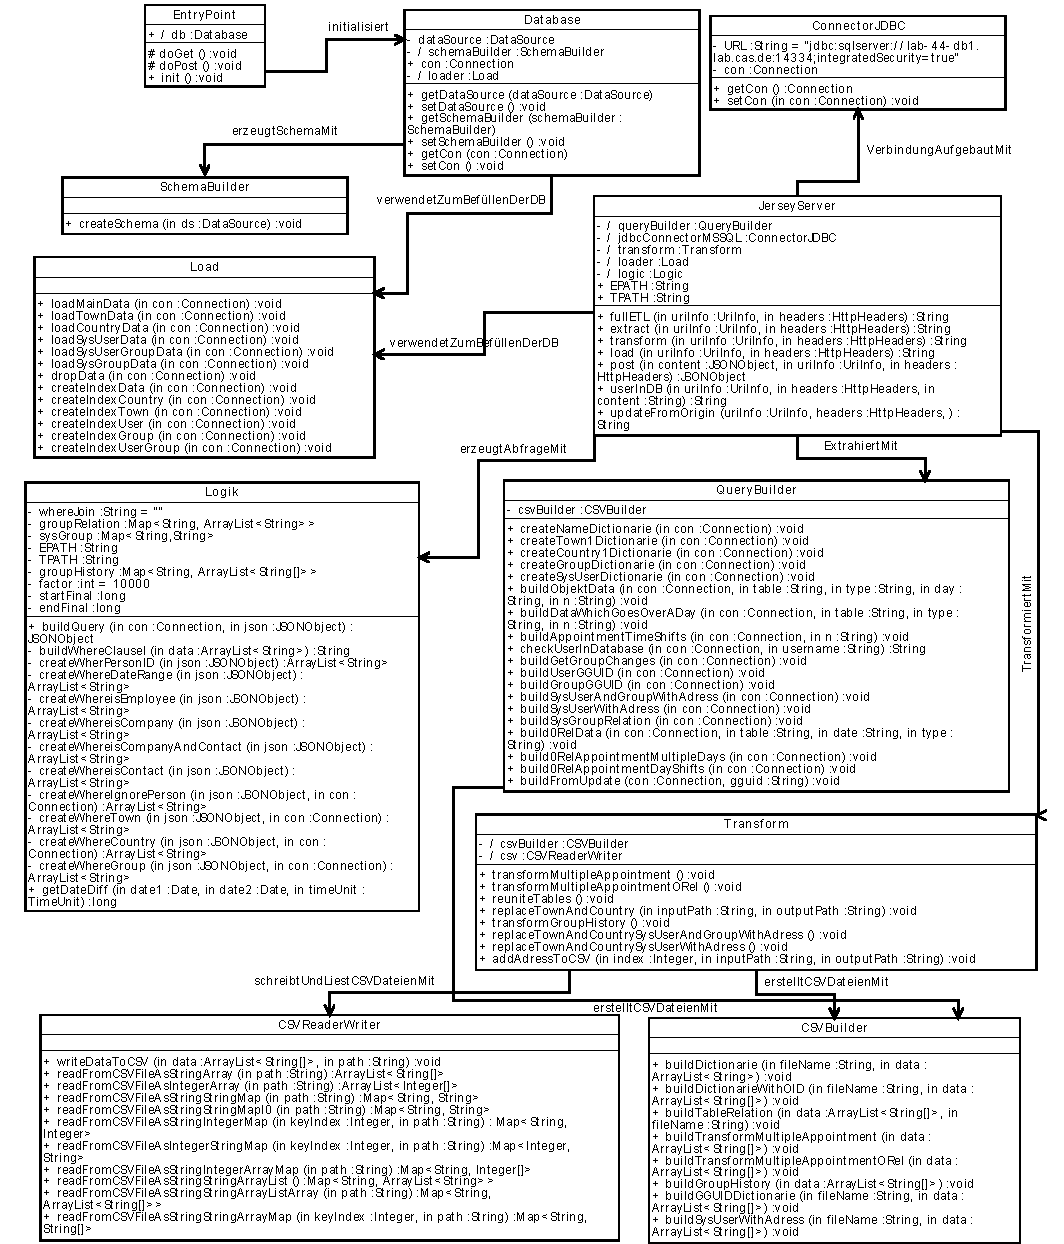
\includegraphics[width=1.0\textwidth]{pics/ServerKlassendiagramm.pdf}
\caption{Server Klassendiagramm}
\label{umsetzung_klassendiagramm_server}
\end{center}
\end{figure}